\documentclass[12pt,twoside]{book}
\usepackage[british]{babel}
\usepackage[utf8]{inputenc}

\usepackage[a4paper,lmargin=1.5in,vscale=0.8]{geometry}

\usepackage{amsmath}
\usepackage{graphicx}
\usepackage{parskip}
\usepackage{natbib}
\usepackage{pgfgantt}
\usepackage{lscape}
\usepackage{pdfpages}
\usepackage{graphicx}
\usepackage{xcolor}
\usepackage[listingsutf8,minted]{tcolorbox}
\usepackage{hyperref}
\usepackage[chapter]{tocbibind}
\usepackage{doc}
\usepackage{minted}
\usepackage{listings}
\usepackage{listingsutf8}
\usepackage[colorinlistoftodos]{todonotes}

\usepackage{fontawesome}

\usepackage{tikz}
\usetikzlibrary{trees}

%
\makeatletter
\def\PY@reset{\let\PY@it=\relax \let\PY@bf=\relax%
    \let\PY@ul=\relax \let\PY@tc=\relax%
    \let\PY@bc=\relax \let\PY@ff=\relax}
\def\PY@tok#1{\csname PY@tok@#1\endcsname}
\def\PY@toks#1+{\ifx\relax#1\empty\else%
    \PY@tok{#1}\expandafter\PY@toks\fi}
\def\PY@do#1{\PY@bc{\PY@tc{\PY@ul{%
    \PY@it{\PY@bf{\PY@ff{#1}}}}}}}
\def\PY#1#2{\PY@reset\PY@toks#1+\relax+\PY@do{#2}}

\@namedef{PY@tok@w}{\def\PY@tc##1{\textcolor[rgb]{0.73,0.73,0.73}{##1}}}
\@namedef{PY@tok@c}{\let\PY@it=\textit\def\PY@tc##1{\textcolor[rgb]{0.25,0.50,0.50}{##1}}}
\@namedef{PY@tok@cp}{\def\PY@tc##1{\textcolor[rgb]{0.74,0.48,0.00}{##1}}}
\@namedef{PY@tok@k}{\let\PY@bf=\textbf\def\PY@tc##1{\textcolor[rgb]{0.00,0.50,0.00}{##1}}}
\@namedef{PY@tok@kp}{\def\PY@tc##1{\textcolor[rgb]{0.00,0.50,0.00}{##1}}}
\@namedef{PY@tok@kt}{\def\PY@tc##1{\textcolor[rgb]{0.69,0.00,0.25}{##1}}}
\@namedef{PY@tok@o}{\def\PY@tc##1{\textcolor[rgb]{0.40,0.40,0.40}{##1}}}
\@namedef{PY@tok@ow}{\let\PY@bf=\textbf\def\PY@tc##1{\textcolor[rgb]{0.67,0.13,1.00}{##1}}}
\@namedef{PY@tok@nb}{\def\PY@tc##1{\textcolor[rgb]{0.00,0.50,0.00}{##1}}}
\@namedef{PY@tok@nf}{\def\PY@tc##1{\textcolor[rgb]{0.00,0.00,1.00}{##1}}}
\@namedef{PY@tok@nc}{\let\PY@bf=\textbf\def\PY@tc##1{\textcolor[rgb]{0.00,0.00,1.00}{##1}}}
\@namedef{PY@tok@nn}{\let\PY@bf=\textbf\def\PY@tc##1{\textcolor[rgb]{0.00,0.00,1.00}{##1}}}
\@namedef{PY@tok@ne}{\let\PY@bf=\textbf\def\PY@tc##1{\textcolor[rgb]{0.82,0.25,0.23}{##1}}}
\@namedef{PY@tok@nv}{\def\PY@tc##1{\textcolor[rgb]{0.10,0.09,0.49}{##1}}}
\@namedef{PY@tok@no}{\def\PY@tc##1{\textcolor[rgb]{0.53,0.00,0.00}{##1}}}
\@namedef{PY@tok@nl}{\def\PY@tc##1{\textcolor[rgb]{0.63,0.63,0.00}{##1}}}
\@namedef{PY@tok@ni}{\let\PY@bf=\textbf\def\PY@tc##1{\textcolor[rgb]{0.60,0.60,0.60}{##1}}}
\@namedef{PY@tok@na}{\def\PY@tc##1{\textcolor[rgb]{0.49,0.56,0.16}{##1}}}
\@namedef{PY@tok@nt}{\let\PY@bf=\textbf\def\PY@tc##1{\textcolor[rgb]{0.00,0.50,0.00}{##1}}}
\@namedef{PY@tok@nd}{\def\PY@tc##1{\textcolor[rgb]{0.67,0.13,1.00}{##1}}}
\@namedef{PY@tok@s}{\def\PY@tc##1{\textcolor[rgb]{0.73,0.13,0.13}{##1}}}
\@namedef{PY@tok@sd}{\let\PY@it=\textit\def\PY@tc##1{\textcolor[rgb]{0.73,0.13,0.13}{##1}}}
\@namedef{PY@tok@si}{\let\PY@bf=\textbf\def\PY@tc##1{\textcolor[rgb]{0.73,0.40,0.53}{##1}}}
\@namedef{PY@tok@se}{\let\PY@bf=\textbf\def\PY@tc##1{\textcolor[rgb]{0.73,0.40,0.13}{##1}}}
\@namedef{PY@tok@sr}{\def\PY@tc##1{\textcolor[rgb]{0.73,0.40,0.53}{##1}}}
\@namedef{PY@tok@ss}{\def\PY@tc##1{\textcolor[rgb]{0.10,0.09,0.49}{##1}}}
\@namedef{PY@tok@sx}{\def\PY@tc##1{\textcolor[rgb]{0.00,0.50,0.00}{##1}}}
\@namedef{PY@tok@m}{\def\PY@tc##1{\textcolor[rgb]{0.40,0.40,0.40}{##1}}}
\@namedef{PY@tok@gh}{\let\PY@bf=\textbf\def\PY@tc##1{\textcolor[rgb]{0.00,0.00,0.50}{##1}}}
\@namedef{PY@tok@gu}{\let\PY@bf=\textbf\def\PY@tc##1{\textcolor[rgb]{0.50,0.00,0.50}{##1}}}
\@namedef{PY@tok@gd}{\def\PY@tc##1{\textcolor[rgb]{0.63,0.00,0.00}{##1}}}
\@namedef{PY@tok@gi}{\def\PY@tc##1{\textcolor[rgb]{0.00,0.63,0.00}{##1}}}
\@namedef{PY@tok@gr}{\def\PY@tc##1{\textcolor[rgb]{1.00,0.00,0.00}{##1}}}
\@namedef{PY@tok@ge}{\let\PY@it=\textit}
\@namedef{PY@tok@gs}{\let\PY@bf=\textbf}
\@namedef{PY@tok@gp}{\let\PY@bf=\textbf\def\PY@tc##1{\textcolor[rgb]{0.00,0.00,0.50}{##1}}}
\@namedef{PY@tok@go}{\def\PY@tc##1{\textcolor[rgb]{0.53,0.53,0.53}{##1}}}
\@namedef{PY@tok@gt}{\def\PY@tc##1{\textcolor[rgb]{0.00,0.27,0.87}{##1}}}
\@namedef{PY@tok@err}{\def\PY@bc##1{{\setlength{\fboxsep}{\string -\fboxrule}\fcolorbox[rgb]{1.00,0.00,0.00}{1,1,1}{\strut ##1}}}}
\@namedef{PY@tok@kc}{\let\PY@bf=\textbf\def\PY@tc##1{\textcolor[rgb]{0.00,0.50,0.00}{##1}}}
\@namedef{PY@tok@kd}{\let\PY@bf=\textbf\def\PY@tc##1{\textcolor[rgb]{0.00,0.50,0.00}{##1}}}
\@namedef{PY@tok@kn}{\let\PY@bf=\textbf\def\PY@tc##1{\textcolor[rgb]{0.00,0.50,0.00}{##1}}}
\@namedef{PY@tok@kr}{\let\PY@bf=\textbf\def\PY@tc##1{\textcolor[rgb]{0.00,0.50,0.00}{##1}}}
\@namedef{PY@tok@bp}{\def\PY@tc##1{\textcolor[rgb]{0.00,0.50,0.00}{##1}}}
\@namedef{PY@tok@fm}{\def\PY@tc##1{\textcolor[rgb]{0.00,0.00,1.00}{##1}}}
\@namedef{PY@tok@vc}{\def\PY@tc##1{\textcolor[rgb]{0.10,0.09,0.49}{##1}}}
\@namedef{PY@tok@vg}{\def\PY@tc##1{\textcolor[rgb]{0.10,0.09,0.49}{##1}}}
\@namedef{PY@tok@vi}{\def\PY@tc##1{\textcolor[rgb]{0.10,0.09,0.49}{##1}}}
\@namedef{PY@tok@vm}{\def\PY@tc##1{\textcolor[rgb]{0.10,0.09,0.49}{##1}}}
\@namedef{PY@tok@sa}{\def\PY@tc##1{\textcolor[rgb]{0.73,0.13,0.13}{##1}}}
\@namedef{PY@tok@sb}{\def\PY@tc##1{\textcolor[rgb]{0.73,0.13,0.13}{##1}}}
\@namedef{PY@tok@sc}{\def\PY@tc##1{\textcolor[rgb]{0.73,0.13,0.13}{##1}}}
\@namedef{PY@tok@dl}{\def\PY@tc##1{\textcolor[rgb]{0.73,0.13,0.13}{##1}}}
\@namedef{PY@tok@s2}{\def\PY@tc##1{\textcolor[rgb]{0.73,0.13,0.13}{##1}}}
\@namedef{PY@tok@sh}{\def\PY@tc##1{\textcolor[rgb]{0.73,0.13,0.13}{##1}}}
\@namedef{PY@tok@s1}{\def\PY@tc##1{\textcolor[rgb]{0.73,0.13,0.13}{##1}}}
\@namedef{PY@tok@mb}{\def\PY@tc##1{\textcolor[rgb]{0.40,0.40,0.40}{##1}}}
\@namedef{PY@tok@mf}{\def\PY@tc##1{\textcolor[rgb]{0.40,0.40,0.40}{##1}}}
\@namedef{PY@tok@mh}{\def\PY@tc##1{\textcolor[rgb]{0.40,0.40,0.40}{##1}}}
\@namedef{PY@tok@mi}{\def\PY@tc##1{\textcolor[rgb]{0.40,0.40,0.40}{##1}}}
\@namedef{PY@tok@il}{\def\PY@tc##1{\textcolor[rgb]{0.40,0.40,0.40}{##1}}}
\@namedef{PY@tok@mo}{\def\PY@tc##1{\textcolor[rgb]{0.40,0.40,0.40}{##1}}}
\@namedef{PY@tok@ch}{\let\PY@it=\textit\def\PY@tc##1{\textcolor[rgb]{0.25,0.50,0.50}{##1}}}
\@namedef{PY@tok@cm}{\let\PY@it=\textit\def\PY@tc##1{\textcolor[rgb]{0.25,0.50,0.50}{##1}}}
\@namedef{PY@tok@cpf}{\let\PY@it=\textit\def\PY@tc##1{\textcolor[rgb]{0.25,0.50,0.50}{##1}}}
\@namedef{PY@tok@c1}{\let\PY@it=\textit\def\PY@tc##1{\textcolor[rgb]{0.25,0.50,0.50}{##1}}}
\@namedef{PY@tok@cs}{\let\PY@it=\textit\def\PY@tc##1{\textcolor[rgb]{0.25,0.50,0.50}{##1}}}

\def\PYZbs{\char`\\}
\def\PYZus{\char`\_}
\def\PYZob{\char`\{}
\def\PYZcb{\char`\}}
\def\PYZca{\char`\^}
\def\PYZam{\char`\&}
\def\PYZlt{\char`\<}
\def\PYZgt{\char`\>}
\def\PYZsh{\char`\#}
\def\PYZpc{\char`\%}
\def\PYZdl{\char`\$}
\def\PYZhy{\char`\-}
\def\PYZsq{\char`\'}
\def\PYZdq{\char`\"}
\def\PYZti{\char`\~}
% for compatibility with earlier versions
\def\PYZat{@}
\def\PYZlb{[}
\def\PYZrb{]}
\makeatother



\begin{document}

\frontmatter
%!TeX root=Dissertation.tex

\begin{titlepage}
\Large
A Report submitted in partial fulfilment of\\
 the regulations governing the award of
\par
the Degree of\\[5mm]
{\huge	 BSc (Honours) Computer Networks and Cyber Security }\\[5mm]
at the University of Northumbria at Newcastle
\par
\vspace*{1in}
{\Large Project Report}
\par\vspace{1em}
{\Huge \bfseries Your Project Title}
\vfill
James Poxon
\par\vspace{1em}
2020/2021
\par\vspace{1em}
General Computing Project
\end{titlepage}

\include{declaration}
%!TeX root=Dissertation.tex

\chapter{Acknowledgements}
I would like to thank my dissertation supervisor Alun Moon for his role in support of my project. I would also like to thank my partner Alex for supplying me endless encouragement throughout the dissertation process.
%!TeX root=../Dissertation.tex

\chapter{Abstract}
Virtualisation is a standard and de-facto technology within server operations, but virtualisation has it's pitfalls, with one of those being the large overheads introduced from virtualisation of a whole operating system. A possible solution to this problem is containerisation. Containerisation runs without a virtualised operating system, instead integrating directly with the host machine's operating system. This effectively removes the OS-component processing overhead required to run each instance of a server, which not only makes servers use less system resources, but theoretically could improve the speed of said servers.

An in-depth analysis into Virtual Machines and Containers was completed to ensure understanding of the problem domain before delving into comparison work of container and virtual machines. It became apparent that most previously published comparison work was specifically aimed at raw hardware performance and utilisation, which whilst useful, doesn't give results relevant to real-world performance.

Two separate but topologically identical computer networks were built. Said topology implemented a primary DNS, two secondary DNS, DHCP, Web, and MySQL servers. One network used VMware (Virtualisation), and the other used Docker (Containerisation) to host the servers. The network topology was designed to be reflective of a possible real-world internal network that we may expect to see in an SME (Small and Medium-sized Enterprise). Four separate benchmarks were then designed, using a mix of different techniques and software, such as JMeter and Sysbench, to accurately test every part of the network.

 Impressive and substantial performance improvements found when moving from VMware to Docker. In some cases, Docker produced over double the output that VMware did. Docker was also found to be far more stable than VMware.

Organisations looking to get extra performance out of ageing hardware could potentially use containers as an alternative to virtual machines for their server infrastructure. However, it is noted Docker is not intended to be used in the way we are applying it. As a result, it was decided that to better support container implementation of servers in the future and to support the transition from Virtualisation to Containerisation, a better, container-based solution for server management should be developed. The benefits of container-based servers are clear to see as a result of this research, but a more server-focused platform that can match the equivalent server-focused virtual machine based platforms that already exist is needed.
\tableofcontents

\mainmatter
%!TeX root=../Dissertation.tex

\chapter{Introduction}


\part{Analysis}
%!TeX root=../Dissertation.tex
%!TeX bibfile=./analysis.bib




\chapter{Review of Virtualisation}

\section{Terminology \& Definitions}


\subsection{Virtualisation}
Virtualisation as a term originated in the 1960s when IBM workers began work on a project that would allow an IBM model-40 computer to segregate off its memory and allow up to 15 users to use the computer independently at once \citep{Lindquist1966}. Each user would see their own abstract Operating System, separate from the others. Whilst virtualisation has continued in its development from this point onwards, the core functionality and architecture behind Hardware Virtualisation, remain much the same.

Each of these individual logical (as opposed to physical) devices is called a `virtual machine'.

\subsection{Hardware Virtualisation}
\label{subsec:HardwareVirtualisation}
There are a number of different types of virtualisation. This can open the scope for what can and can not be considered as a virtual machine. For the purpose of this report the term `virtualisation' will refer specifically to `hardware based virtualisation', whereby a `virtual machine' is an operating system running on top of another operating system, with the virtualisation task itself being controlled by a `hypervisor' (This is explained in more detail in the next subsection: \ref{subsec:hypervisor}).

This is an important definition to clarify, as often times containerisation (subsection \ref{sec:containerisation}) can be viewed as a type of virtualisation, and other times not. For the purposes of this report, the two definitions must be distinguished as separate things, much like in the report ``Autonomic Orchestration of Containers: Problem Definition and Research Challenges'' \citep{casalicchio2016}, where a clear and defined difference between Hardware Virtualisation and Containerisation is made.

\subsection{Hypervisor}
\label{subsec:hypervisor}
Hardware Virtualisation relies on an underlying software that runs on the already existing OS in order to manage each instance/OS. This software can have a number of different names depending on the origin of the work, and the context. In early work on virtualisation, this software was often referred to simply as a ``control program'' \citep{creasy1981}, but for the purposes of this research, this software will be referred to as a `Hypervisor'. This term is often preferred in practical settings, such as in VMware's online Glossary \citep{vmwareHypervisor}, or in Red Hat's ``What is a hypervisor'' \citep{redhat2021}.



\section{The workings of virtualisation}
Virtualisation works






\chapter{Review of Containerisation}


\section{Terminology \& Definitions}

\subsection{Containerisation}
\label{subsec:containerisation}
Containerisation has become the de-facto term to describe what could also be described as OS-level virtualisation. For the purposes of this report, I will be referring to this technology only as Containerisation, and each individual instance as a container (instead of virtual machine). This is the same approach towards defining containers as taken by Dua et al \citep{dua14} when they have made their own distinction between Containers and Virtual Machines.

\subsection{Container Engine}
\label{Container Engine}
What a hypervisor is to a virtual machine, a container engine is to a container. A container engine sits on the base operating system, much the same as a hypervisor. Where a difference is found however, is in the way it interacts with the base operating system.

Whilst a hypervisor works by running a full operating system on top of the existing one, a container engine works without that upper operating system by using the base operating system as the OS component for each container. Segregation of containers and resource allocation is simply managed by the container engine, so that each container is allocated resources. This can be done dynamically or be static, depending on the use-case.




\section{Developments in containerisation technology}

\subsection{Docker}
A now ever more popular implementation of container technology is a software known as Docker. This software is primarily used (and aimed at) app developers, who can use the platform to quickly create and deploy applications for businesses. The use of containers is supposed to make managing these applications much easier, and ensures compatibility along the whole development process.
Datanyze (a technology market usage group) report that Docker is currently the second most used Containerisation platform, with 25.34\% market share in Containerisation \citep{datanyze}. 

Docker's Container engine is aptly named Docker Engine, and utilises a client-server architecture \citep[Section: Docker architecture]{DockerOverview}. The server portion of the Docker System is known as the `docker daemon', the Client uses a command line interface to interact with one or more docker daemons. The client and daemon communicate using a `REST API' \citep[Section: The Docker daemon]{DockerOverview}. REST (Representational State Transfer) provides an architecture for web services \citep{W3Architecture2004} that allows them to communicate. The protocols within REST are stateless, this means there is no set `state' or session control within the protocol. REST API being used as the communication method between the Docker Daemon and the Client means that each command sent to a daemon can be understood as it is, without the need for any outside context to the command being sent.

The Docker Daemon manages Docker the various `Objects' \citep[Section: Docker objects]{DockerOverview} required for a full Docker system. These include the containers, the images (Docker images are the instruction sets for Docker containers, not to be confused with OS images) and the Registry, which acts as a storage for the Docker images.







\chapter{System design and definition}


\section{Maintaining scientific method}
To ensure that results are scientific, variables must be controlled between both of the systems. The first step in this, is ensuring that the topology and configurations for both systems are the same. This can be done by copying the configuration files from one system to the other, ensuring that the system works in the same way for both systems. As the underlying operating system should be a version of Linux for both the virtual machine and the Docker system, this should be relatively easy.

To further ensure that variables are controlled, we need to ensure that the same benchmarks are maintained throughout the testing process, when being used on the \emph{same part of the system}. This means that if one benchmark is used to measure, for example, network latency on a web-server, then the same benchmark should be used to measure the network latency on that same web-server on the mirrored system. It may be necessary to use different benchmarks across the whole system, but this is acceptable as long as all testing is done to a parallel across both systems. The benchmarks to be used will be discussed in more detail in subsection \ref{sub:Benchmarking} (Benchmarking).

\subsection{LAMP System}
In order to make sure that the system is as accurate tom a real-world system as possible, a full LAMP topology will need to be implemented for both the Docker system and the Virtual Machine system. LAMP is the acronym of Linux, Apache, MySQL and PHP, whilst this can technically be run on one system, it is common to separate various functions out onto different logical machines, this generally makes management of these systems easier, and often more streamlined.

\subsection{Benchmarking}
\label{sub:Benchmarking}
Benchmarking software and tools are designed to create a standard output measurement for performance of a computer-based system\citep{fleming1986}.

There are a great number of benchmarking tools available to me for this research, but generally these can be split in discussion along lines of what exactly they are designed to measure. The main split for this research, being the measuring of base compute performance, and of network performance.

\subsubsection{Base Computing Performance}
Base computing performance in this case relates to the performance as a result of the computers ability to process information, and at what rate. Whilst this is tied directly to the processor, RAM, and other hardware, the Operating system itself can also have a large affect on the performance of a system, as it will always take up an amount of utilisation over time. This effect is known as `operating system overhead'. Based on previous research on containers and virtual machines it can be hypothesised that the total Operating System overhead for a container-based system will be smaller than that of Virtual Machines \emph{(when using the same operating system)}. This is simply due to the way that containers utilise one OS for their function (as discussed in subsection \ref{Container Engine}).

\subsubsection{Network Performance}

\subsection{DNS}

\subsection{Webserver}

\subsection{Intranet}

\chapter{How will the system be measured}
%Talk about benchmarks.

\part{Synthesis}
\include{synthesis/synthesis}

\part{Evaluation}
\include{evaluation/evaluation}

\part{Conclusion \& Recommendations}
%!TeX root=../Dissertation.tex
%!TeX bibfile=./synthesis.bib
%!TeX bibfile=./analysis.bib
\chapter{Conclusions}
%MAIN THING HERE IS COMPARING TO THE AIMS
\section{Main Test Result Conclusions}
The primary aim of this research was to measure performance between Containerised and Virtualised network infrastructure, with the hope of generating recommendations to either those that already use virtual machine infrastructure, or to those that are creating new headless servers and wondering which option to use.
With that in mind, I can confidently say that the total output from this work has been a success. A number of in-depth tests have been done to generate a solid set of results. These key and conclusive results are as follows:
\begin{itemize}
  \item Docker, when being used to run headless servers, performs faster than the same servers perform on a VMware machine.
  \item Docker can provide in most cases, over double the performance output when compared to VMware for the same workload.
  \item Docker uses far less system resources when compared directly with VMware.
  \item Docker's performance is more stable and reliable than VMware under load.
\end{itemize}

\section{Secondary Points of Interest}
%Talk about the ways that Docker is managed, and the ways that VMware is managed.
Other interesting points of discussion are also relevant, but less important than the main discoveries that are laid out above. One of these discussion points sits with the way that Docker and VMware are both managed. These two different methods are not exclusive to containerisation or virtualisation respectively, but when making recommendations based on the work done in this research, these points are still important to mention.
\begin{itemize}
  \item Docker is managed firstly from the command line. Dockerfiles can be written to quickly create new Docker Images, or, Images can be pulled directly from Dockerhub or a private repository. Images that are already created can be saved to .Tar files, or can be pushed to a repository. Multiple containers can use the same image, as IP addressing is done when launching a container. Networks which bridge to real interfaces must be created and defined by the user, using Docker's macvlan network driver. Macvlan is not the primary, or most supported network option provided by Docker.
  \item VMware is managed using VMware's workstation software. Virtual machines must either be created using the setup wizard using a real OS image file, cloned from another machine (If the original machine is deleted or lost, the clone will fail), or a direct copy of the VM can be created (by manually copying the Virtual Machine files). VMware comes ready with a `bridged' network, along with virtual networks that can connect with other services via adapters. The bridged network option is well supported by VMware.
\end{itemize}

I believe these are important points to mention as they should be considered by anyone that is planning on using this research to form an opinion about which technology to use. Neither of these methods is the right or wrong way of managing containers and virtual machines, but as they are different, it may still be an important basis for that persons decision making. For example, Docker's command line interface could for some end users such as network administrators be a feature they prefer over VMware's GUI interface. On the other hand, those with less technical knowledge might find VMware more user friendly. Another example is the way that Containers and Virtual Machines are stored. Both allow ample opportunity for backups, and rapid redeployment of server solutions should the need arise (though it could be argued that Docker is faster). These points are less quantitative, and more qualitative it is entirely up to the end user as to what matches their needs.

That being said, I do think that VMware's solution is more user friendly even if hardcore IT users may prefer a CLI over a more GUI. Someone with CLI knowledge may prefer that as an option, but they certainly wouldn't struggle to use VMware. The same could not be said the other way around. Docker is first and foremost a low resource solution, and as such should be used from the Command Line. Docker does have a `Docker Desktop' version that works on Windows and Mac, but this version uses different techniques to simulate the containers (for example, on windows it uses Windows Subsystem for Linux \citep{DockerWindows}), and as such we can't make recommendations for these versions of Docker, as there may be other constraints on container performance.

It is also important to talk here about the way that Networks are managed in both solutions. Docker's networks are generally configured by the user (a default virtual network is provided but not recommended). For containers to face a real network, the macvlan driver is used. This network mode isn't the most supported network option, and there can be problems regarding the handling of some IP traffic. This is evidenced by the issues around DHCP that we experienced in subsection \ref{Difficulties with Docker and DHCP}. When looking at VMware, the network management is far more robust. The systems that VMware uses to bridge virtual machines to real networks are far better supported, and for all intents and purposes, function exactly like a real machine would.


%Most of the issues come from having the hostmachine being one PC, results of covid and not having access to infrastructure at university. I was to do it again the most important step would be to run the test on a server machine on a real network. This test more a simulation than real life.

\section{Rounded Conclusion}

To sum up, Docker is a far better option than VMware when looking solely at performance metrics and resource usage. VMware was far slower, and as a result of it's high resource utilisation, it suffered fluctuation making it less reliable under load. However, Docker isn't designed around this kind of use, and as a result can suffer from being less straight and operable. VMware provides a more robust system for managing its instances. VMware's Bridged network mode is also more desirable than Docker's macvlan mode. 

It is clear that more work needs to be done to provide a suitable base for containerised networking specifically. The performance benefits to using Containers over Virtual Machines is a one that should be utilised, but Docker, as it stands now, probably isn't the best way forward. Should Docker want to provide this as a part of their platform in the future, they need to work on better ways to implement containers with real networks.

I am sure that once these issues are ironed out, that container based networking will be the future. I would hypothesise that we will start to see less and less virtualised infrastructure in favour of containers simply due to being able to get the same performance out of lesser hardware (something that will save costs).
%Actual conclusion is: Docker performs better than VMware, uses less resources, but there is still work to be done to make Docker more accessible, and to make it integrate with networks better. Once these issues are ironed out, containers will be the future.

\chapter{Recommendations}

\section{For those considering moving to Containers}
\label{sec:RecSMEs}
This section will comprise of information and recommendations to those that may want to use this research as part of their decision making process about moving to Containers to support their network infrastructure. Whether that be moving from virtual machines to container on an already existing machine, or whether it be part of a decision as to which technology a new system should be using.

The performance results in this report speak for themselves. Docker \emph{is} the superior choice if performance and reliability is the only metric that matters to you or your organisation. If there are no other considerations for your use-case, then the recommendation here would be that containerisation is absolutely the correct choice. However, it would be very unlikely that these are the only considerations. Security, Cost, Ease of Use, and Management Options are all important aspects to consider when deciding how to host network infrastructure.
\subsection{Security}
\label{conclandreccoSecurity}
Security in computing is often split into the CIA triad (Confidentiality, Integrity, Availability). Lets split both the technologies (Docker and VMware), along with the results we have collected, into the CIA triad, and see how they compare.
\subsubsection{Docker}
Confidentiality is something we didn't investigate during this research, but it has been suggested by other research that isolation is a problem with Docker. I would strongly recommend anyone planning on moving to Containers to read the paper by \citeauthor{watanda19} ``Emerging Trends, Techniques and Open Issues of
Containerization: A Review'' (\citeyear{watanda19}). This paper covers security and isolation concerns with containerisation which are important but outside of the scope of this research.

When we move to Integrity, we can comfortably say that this research tested this well, and we find that Docker's integrity stands up under scrutiny. The servers and services hosted via Docker were reliable and stable, and could hold up even when under heavy loads and stress testing.

Availability was also tested during this research. All the systems stayed up and running at reasonable levels throughout testing, with only minor hiccups that we would expect to see in any operational system anyway.

\subsubsection{VMware}
Again, we haven't touched on Confidentiality in our study as it was outside of our scope. However, VMware's isolation from the host machine, and between virtual machines is very well documented. For example; \citeauthor{VMwareIsolation} discusses this in their ``Survey of security isolation of virtualization, containers, and unikernels'' (\citeyear{VMwareIsolation}).

Where our research does interject is when looking at Integrity of data. The processing we saw in our tests, namely the database test (where important data would most likely be exchanged in a real system) showed that we had scattered results where we would observe very high latencies. As discussed in our evaluation, these were probably due to errors. The number of these errors we noticed was significantly more than that of Docker. So if you are planning on using VMware to host mission critical infrastructure, we would remind you that VMware may introduce these hitches that could be detrimental to the integrity of your data.

Availability is another area affected by VMware observed performance hits. The fluctuation caused by this lack of performance in our tests could result in end users sometimes not having access to systems during peak times, as sudden drops in performance happening quite often. This is not acceptable for any system that need to be used by a number of users. 

\subsubsection{Recommendation based on security}
Our recommendation, then, would be that should Confidentiality be the main priority of your system, Docker is probably not the solution for you. If Integrity and Availability of your data is more important to you though, then we would recommend Docker over VMware.

\subsection{Costing}
Another interesting point to mention here is cost of applications. VMware Pro (which is required to use the network manager) is part of a paid software package, whereas everything we did in our tests was possible using Docker's free plan. It is more than possible that however that businesses using Docker may want private repositories or other features that are only provided in Docker's paid plans. It is also possible, that an organisation using VMware, may not require access to the network manager, as bridged connections shouldn't require much (if any at all) configuration. The cost difference's between the two technologies at this point then simply comes down to the preference and requirements of the organisation setting out to use either of the technologies.

\subsection{Concluding recommendation}
From what is discussed in the sections above we can see that the use of VMware or Docker isn't clean-cut. It entirely comes down to the individual needs and requirements of the entity that is requiring a network solution. So whilst our study does a lot to prove the efficiency and performance benefits of containers, it cannot be used as the sole indicator of whether you should used Containers over Virtual Machines.

This moves us onto our next, and final section.

\section{Suggestions for further research and development}

%Recommendation up here first, then development opportunities (already written some of it) below that.
%Most of the issues come from having the hostmachine being one PC (you have talked about this above, this is just the recommendation, nothing else.

As discussed in the section above (Section \ref{sec:RecSMEs}), there are multiple reasons other than performance that come into the adoption of a new technology. Someone could develop the fastest database system in the world, but there would be very little uptake on the technology if it was also the least secure database system. End users need the reassurance that the systems they implement are right for them, and I don't yet feel fully confident in recommending container based networking, as I feel there are still issues that need to be addressed.

For full recommendation of Docker as a tool to host and run networks, it is clear there is work to be done. Firstly, Docker needs to do more work to offer flexibility in it's networking solutions. The macvlan adapter support is simply not good enough, or reliable enough to recommend as a long-term solution on a real network. Secondly, Docker should look to implement a more top-down management view of their containers, that allows end-users mass control over container networks in a similar way as is already possible on Virtualised networks. Furthermore, a deeper focus on the security implications would give end-users the confidence they need when hosting critical servers. Should these few sticking points be straightened I would be able to not only offer Docker as a better alternative in all ways to VMware, I would happily suggest that moving away from Virtualisation and into a new paradigm of Containerisation is inevitable. In-fact, despite the issues listed here, I am almost sure that containers are the future of single-machine networking.

Maybe the issue is that Docker was never designed to be the tool we are trying to turn it into. Docker was created firstly as a way for developers to easily host their applications for testing. It wasn't designed to be used as a permanent networking solution. With that in mind, my recommendation would be that a networking-focused container based solution need to be developed, from the ground up. I believe that a purpose-built containerised network solution, that addressed the issues discussed in this paper such as real world network cross-over, or security and isolation, would find themselves as a new leading industry standard. I also have no doubt that various Virtualisation and Containerisation solution providers are already working on these kinds of solutions. We are already starting to see uptake of containerisation in areas such as Platform as a Service (PaaS), whereby containers \emph{are} being used in an online environment, in order to provide cost-effective application environments \citep[Page 55]{PAASCloudBook}. %FINISH THIS TODO.
%FINISH THE BIT ABOVE
%FINISH THE BIT ABOVE
%FINISH THE BIT ABOVE
%FINISH THE BIT ABOVE

\bibliographystyle{plainnat}
\bibliography{TermsOfReference/tor, analysis/analysis, synthesis/synthesis, AbstractAndIntroduction/introduction}


\part{Appendices}
\appendix

\chapter{Terms of Reference}
\label{appendix:tor}
%!TeX root=TermsOfReference.tex

\section{Background}
Virtualisation has been utilised by a number of industries for a long time now, with first iterations of virtual machines dating back to IBM in the 1960s \citep{pugh95}. System Virtual machines allow an operating system to emulate the function of a full operating system layered on top of a base operating system. Functionally, this allows multiple different logical 'computers' with varying operating systems to run on one physical computer. In most modern implementations, virtualisation requires software (known as a hypervisor) to manage and create the virtual machines.

Whilst I was on a year-long placement provided as part of a sandwich course at my university, I had the chance to work in an IT risk department at a reputable enterprise in Newcastle Upon Tyne. whilst working there I witnessed first hand, infrastructure and operations departments using virtualisation for much of the internally and externally facing server infrastructure, in what was an unwieldy and cumbrous use of scripts to update and install patches and dependencies across a multitude of systems. This resulted in a number of incidents where systems had to be pulled down in order to update the Operating Systems of individual virtual machines. These methods often caused unnecessary down time for systems, resulting in substantial risk for the business. Furthermore, this method often put a substantial stress on the hardware of these systems, with hardware boxes often running at full resource potential under heavy load, and whilst these boxes were designed to withstand these kinds of loads, it still affected the longevity of the hardware.

In recent years there has been research into the use of containers instead of virtual machines for various operations across computing industries \citep{watanda19}. Containers are different from virtual machines in that they run on the base OS, and don't require a secondary emulated operating system to be managed by a hypervisor. This is a benefit as it reduces the resources \citep{joy15} used by each instance. Overall, containers are a more lightweight and efficient system, that are easier to keep up to date. Whilst research has claim in displaying the benefits of containerisation, much of the server infrastructure of enterprise remains reliant on Virtualisation, not Containerisation.

I have also had the opportunity to partake in gatherings held by CoTech, a network of tech co-operatives that meet semi-regularly to discuss various tech related topics. Whilst I was there, it was discussed that a large portion of these small enterprises used Docker, a system for packaging and deploying containers, to develop applications for their clients.

There is historical research that compares virtualisation and containerisation for other technical applications, for example \citep{dua14} compares the two methods inside the context of PaaS (Platform as a service), which is similar to co-techs use of Docker. It seems that the application for containerisation has been realised as early as 2014 when it is being applied to the development and hosting of applications, but not as much when talking about the running of wider server infrastructure. This is further supported by research from '451 Research' who in 2017 estimated a compound annual growth rate of 40\% for containers in 2020 \citep{451}, suggesting a coming paradigm shift from virtualisation to containerisation.

\section{Proposed Work}
\label{proposed}
I plan to do similar work to the studies I have already mentioned \citep{joy15}, \citep{dua14}, but instead focus this work on my own context and my own interest in Operating Systems and Server Infrastructure. I have experience with running headless servers on virtual machines already, through the Advanced Operating Systems module I did in my second year of study at Northumbria University. 

It is important to set a baseline system here, and to best reflect a realistic topology, I will use LAMP (Linux + Apache + MySQL + PHP). I have experience with Ubuntu server, so I will use this version of Linux as the base operating system for my virtual machines, and plan to host a full working topology of servers, including a DNS architecture, a web-server architecture that includes HTTP (Apache) servers, NFS servers and MySQL servers. The reasoning for doing this is to create as realistic a topology as possible, and to ensure a somewhat realistic level of network traffic so that meaningful data can be captured.

For the virtual machines, I will use the virtual machine infrastructure available to me through the university, and for the container infrastructure, I plan on using Docker. This is because Docker is a popular choice among app developers, and is supposed to make container deployment easy. Though, as I have never worked with containers before, if Docker fails to be a good way of providing containers for web-servers, then there are a number of other ways to deploy containers, such as LXC, that I could turn to as a contingency.

I will also need to set a standard for measurement to ensure that my data is meaningful and uses the scientific method. I plant to use tools such as iPerf3 (for network performance) and Sysbench (for hardware performance) across a number of servers. It is important to measure both network and hardware performance (CPU, Memory, Disk, etc) to ensure that described  benefits are achieved for the system as a whole. iPerf is an industry standard tool for measuring network performance on Linux systems, whilst Sysbench is a full benchmarking suite for linux that will let me benchmark the CPU, file IO, and importantly, MySQL performance (allowing direct measurement of database performance on the machine that will be hosting the previously mentioned MySQL database. Whilst I have mentioned these benchmarking tools, it is possible that they could have problems with integrating with certain applications or environments, in this case, there is a number of other standard benchmark utilities (Phoronix Test Suite, KDiskMark, UnixBench, etc) available that should give me the flexibility to create measurements. Whilst these utilities all have differing overheads within them (meaning they will use up varying resources to run the benchmark), as long as I use the same benchmark across the same machines I am comparing, this overhead shouldn't effect the measurable performance difference between these machines.

Once data is collected, I will do a comparative analysis of the data to determine if there is a clear improvement as previous research suggests, and if this difference is enough to justify a change in the current best-practice use of virtualisation.

\section{Aims and Objectives}

\subsection{Aims}
\begin{quote}

To compare and contrast the performance difference and hardware impact between virtualisation and containerisation when running headless servers.

\end{quote}

\subsection{Objectives}
Your objective list is a series of measurable objectives, can you tick each one off as \emph{done}?  I usually expect between 8 and 12 objectives

\begin{enumerate}
	\item \label{itm:problemdomain} \textbf{Explain the problem domain that encompasses current practices in virtualisation.}
	\item \label{itm:explainmethods} \textbf{Explanation of the two different methods in practice.}
	\item \label{itm:softwarehardware} \textbf{Determine the software and hardware to be used.}
	\item \label{itm:infrastructure} \textbf{Design the network infrastructure to be built.}
	\item \label{itm:learndocker} \textbf{Learn how to implement and utilise containers using Docker.}
	\item \label{itm:buildvirtual} \textbf{Build the network topology on the virtual machines.}
	\item \label{itm:buildcontainer} \textbf{Build the network topology on the container system.}
	\item \label{itm:determinemethod} \textbf{Determine a method to scientifically evaluate and determine performance of both systems.}
	\item \label{itm:measure} \textbf{Accurately measure performance of the two systems.}
	\item \label{itm:comparison} \textbf{Compare and contrast between the findings for both systems to determine improvements or failings.}
	\item \label{itm:conclusion} \textbf{Create a recommendation regarding the real-world implementation of containerisation in this use case.}
\end{enumerate}

\section{Skills}
This is where you can cover the skills you have relevant to the project and the new skills you are going to acquire during the project.
\begin{enumerate}
	\item Advanced Operating Systems 1, see module KF5004.
	\item Computer Networking Experience.
	\item Computer Technology, see module KF4004.
	\item Virtual machine configuration.
	\item LAMP topology experience.
	\item Docker configuration.
\end{enumerate}

\section{Resources}
I will require access to Virtual Machine infrastructure in order to do build my topology and compare virtual machine performance.
I will also require access to a machine that has the same hardware and system resources as those shared by the virtual machines, as I will need to perform my containerisation tests on the same hardware in order to effectively control that variable.

\subsection{Hardware}
I shouldn't require any hardware as long as I can get remote access to the virtual machine infrastructure in a way that allows me to use the same resources for containerisation (as mentioned above).

As contingency, if I cant access this infrastructure, I will still need some way of creating and managing virtualisation. This might be possible on my own hardware, though I'd rather use university infrastructure as this should be more reliable and accessible.

\subsection{Software}
I will need to install Docker, and will need access to benchmarking suites, but these are free and/or open-source.

\section{Structure and Contents of the Report}
Below I will set out the chapters that I will most likely have in my final report.
\subsection{Report Structure}

\paragraph{Abstract \& Introduction}  Here I will set out the background for my project and the reasoning behind the work I will be doing. The Abstract will also summarise the work that has been done along with my findings, subsequent recommendations and conclusions.

\paragraph{What is virtualisation \& containerisation} An introduction to virtualisation and its current context and usage in today's world of computing. An introduction to containerisation, what it is, how it works, and how it differs to virtualisation. This will form part of my literature review.

\paragraph{Current uses of virtualisation} An explanation of modern uses of virtual machines. I will emphasis virtual servers here, and the reasons they are used.

\paragraph{Current uses of containerisation.} An explanation of modern usage of containers. I will emphasise application development and other, non-main-sever applications here.

\paragraph{Application of containerisation to server infrastructure} Introduce the idea of applying containers to the area I study, with the use-case of server infrastructure. Explain what the implications of this could be. Set out a detailed definition of the problem I want to solve/test. Brief explanation of how this could be designed, with reference to other similar studies.

\paragraph{Network Infrastructure Design} Here I will lay out the infrastructure that I want to implement for my testing and my reasoning for this, along with references \hyperref[proposed]{(see proposed work)}.

\paragraph{How to test and measure the system} Justify the creation or use of a particular set of benchmarks that I will use against the system for testing. I will also explain here how I will measure and evaluate the two systems.

\paragraph{Building the Virtual System} Here I will build the virtual system to work with the topology laid out in the infrastructure chapter. I will make sure to explain how to do it. I will also provide evidence of the system working.

\paragraph{Building the Container System} Similar to the previous chapter, I will build the container based system following the topology laid out in the infrastructure design section. I will explain how this is done. (ie, using Docker). \hyperref[proposed]{(see proposed work)}. As per the previous chapter, I will provide evidence of this working in practice.

\paragraph{Testing and gathering data} Here I will create a test plan for running benchmarks across the parallel servers in order to compare the like for like running of both systems.

\paragraph{Analysis \& Comparison} I will briefly explain how the data shown was required as an introduction to what the data shows. This is where I will explain in detail the actual results, and what they mean, I won't infer here.

\paragraph{Evaluation of the system} A technical evaluation of the system I created. I will highlight and strengths, and failings in my ability to meet the requirements of my implementation. I will also ensure to evidence this accordingly.

\paragraph{Evaluation of the project process} Here I will evaluate my own learning, and explain what I would do differently about my approach, should I go on to do the same, or a similar, project in the future. My objectives should be assessed as per the marking scheme laid out in the project handbook.

\paragraph{Conclusion and Recommendations} I will first create a balanced conclusion, considering the main points mentioned in my evaluation sections. This should cover the direction the work went in, presenting key findings as a way of getting my opinion on the project across. I will present my opinions on the usage of containers in practical setting (ie, whether I think they should be used instead of virtualisation; where they would/could be used) Furthermore, as my work should have practical implications on enterprise and organisations that use virtualisation, I will aim to create recommendations of further work in order to push this area further in the future.

%analysis section Chapters: what is network infrastructure I want to model (analysis chapter), design work of the two implementations. Could include creation/justification of benchmark (made one or found one)

%Synthesis chapters: Build the systems, run and gather the data, analyse the data.

%Lift sections from handbook for the evaluation.

\subsection{List of Appendices}
My appendices will first include my TOR, Ethics form and Risk Assessment.

Some of the network design documentation may be included if too large for the main body, along with the configurations from the various servers.

I should also include the full and direct results of my benchmarks, as these will almost certainly be too large to display in my main text. (I will instead pull the direct numbers from the benchmarks and reference to the related Appendix).

%What Appendices you will include.  A copy of the TOR should be the first, followed by the Ethics form and the Risk Assessment.

%Others might include design documentation, code listings, tables of results (if too large to include in the main text).



\section{Marking Scheme}
The marking scheme sets out what criteria we are going to use for the project.

\paragraph{Project Type} General Computing.

\paragraph{Project Report}
\emph{Analysis Chapters}
\begin{itemize}
	\item What is virtualisation \& containerisation.
	\item Current uses of virtualisation.
	\item Current uses of containerisation.
	\item Application of containerisation to server infrastructure.
\end{itemize}

\emph{Synthesis Chapters}
\begin{itemize}
	\item Network Infrastructure Design.
	\item How to test and measure the system.
	\item Building the Virtual System.
	\item Testing and gathering data.
	\item Analysis \& Comparison.
\end{itemize}

\emph{Evaluation Chapters}
\begin{itemize}
	\item Evaluation of the system.
	\item Evaluation of the project process.
	\item Conclusion and Recommendations.
\end{itemize}

\paragraph{Product} The 'product' includes the Network Infrastructure design, the configurations across both systems, the virtual system and the container system themselves.

% List the deliverables that make up the 'Product'.  Code, design, requirements specifications, test plans, etc.

%For the 'Fitness for Purpose' and 'Build Quality'  list the criteria used to asses the product by.

\subparagraph{Fitness for Purpose}~
\begin{itemize}
	\item Meet requirements identified.
	\item Application to real world infrastructure.
	\item Whether the headless servers can communicate effectively on both systems.
	\item Whether both systems achieved the same goals and outcomes. They should have the same logical topology.
\end{itemize}

\subparagraph{Build Quality}~
\begin{itemize}
	\item Requirements specification and analysis.
	\item Quality of the infrastructure design.
	\item Configuration quality.
	\item Benchmarking plan quality.
\end{itemize}

\clearpage

\section{Project Plan}
\noindent
\rotatebox{90}{%!TeX root=TermsOfReference.tex

% A lot of the settings here are tuned to fit a landscape gantt chart into
% an A4 piece of paper.
\begin{ganttchart}[
time slot format=little-endian,
calendar week text=\currentweek,
x unit=2.4pt,
y unit chart=14pt,
y unit title=12pt,
title label font=\scriptsize,
bar top shift=.15,
bar height=0.7,
milestone label font = \small,
group label font = {\tiny\bfseries},
group inline label node/.append style=centered,
hgrid=true,vgrid={*6{draw=none},dotted},
region/.style={inline,group peaks width=2,
  group peaks height=0.25, group height=0.5,
  group top shift=0.2 ,group/.append style={fill=#1}},
milestone left shift=0,
milestone right shift=1,
ms/.style={inline,
    milestone inline label node/.append style={#1=0pt}}
]%
% For semester dates see
% https://www.northumbria.ac.uk/about-us/university-services/academic-registry/registry-records-and-returns/academic-calendars/
{21/9/20}{28/05/21} %<- Dates Gantt Chart runs from and to

\gantttitlecalendar{year,month,week=1}\\

% Highlight Smesters and Vactions
\ganttgroup[region=blue!20]{Semester 1}{21/9/20}{22/1/21}
\ganttgroup[region=blue!50]{Semester 2}{18/1/21}{28/5/21}\\
\ganttgroup[region=red!50]{Christmas}{21/12/20}{8/1/21}
\ganttgroup[region=green!25]{Easter}{29/3/21}{16/4/21}\\

% Project Deadlines (from the Project Handbook)
\ganttmilestone[ms=left]{PID}{12/10/20}
\ganttmilestone[ms=left]{final \bfseries TOR}{16/11/20}
\ganttmilestone[ms=right]{Draft Analysis}{30/11/20}
\ganttmilestone[ms=left,milestone/.append style={fill=red}]{\bfseries Submit}{29/4/21}
\ganttnewline[thick]

% --Tasks go here
% put in a title, a start date, end date...
\ganttbar{TOR}{28/9/20}{26/10/20}
\ganttbar[inline]{\emph{revise}}{28/10/20}{16/11/20}\\
\ganttbar{Analysis}{30/9/20}{24/11/20}\\
\ganttbar{Design}{31/10/20}{19/1/21}
% Note how you can refer to labels set in the objectives list!
\ganttmilestone[ms=right]{Build complete (Obj \ref{write-code})}{18/1/20}\\
\ganttbar{Exploration}{22/10/19}{15/1/20}
\end{ganttchart}

}
 %<- note use of \input{} not \include{}

\chapter{Test Data}
\section{Test One - iPerf3}
\subsection{VMware Client}
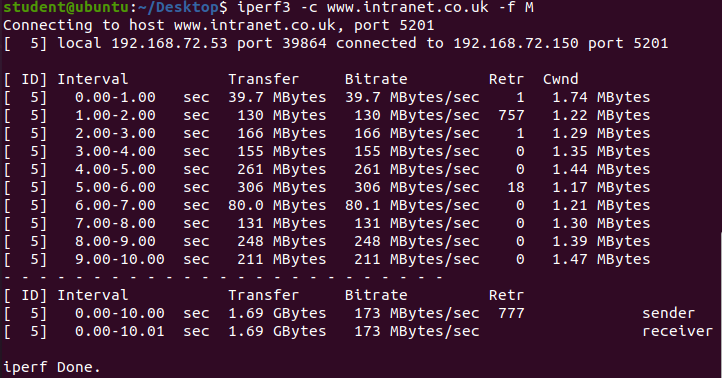
\includegraphics[width=0.80\textwidth]{Appendicies/VMwareTest1Client.PNG}
\subsection{VMware Apache Server}
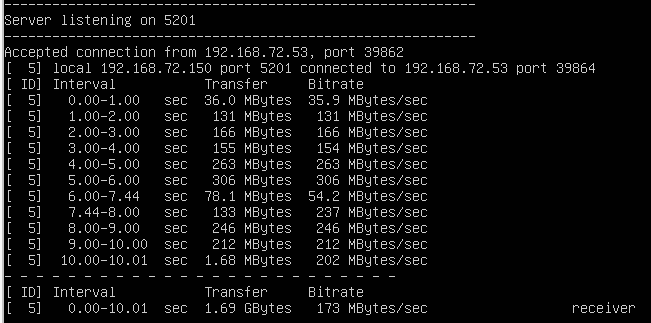
\includegraphics[width=0.80\textwidth]{Appendicies/VMwareTest1Apache.PNG}
\subsection{Docker Client}
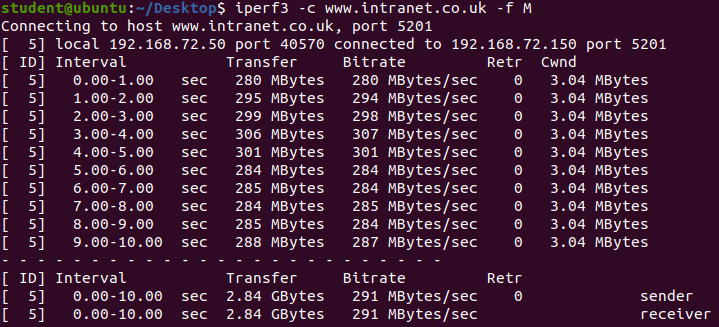
\includegraphics[width=0.80\textwidth]{Appendicies/DockerTest1Client.PNG}
\subsection{Docker Apache Server}
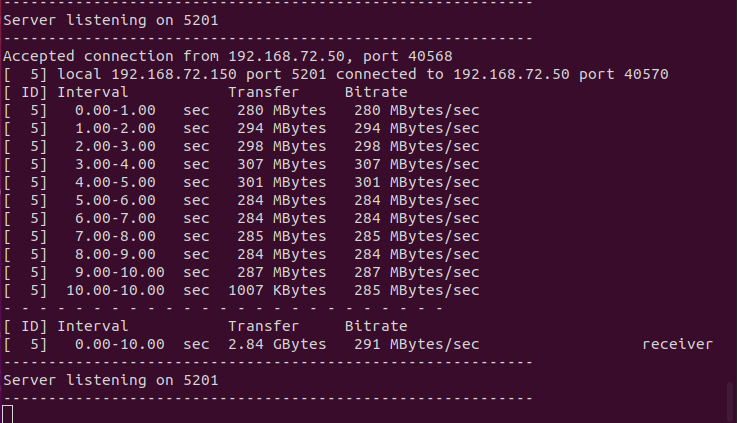
\includegraphics[width=0.80\textwidth]{Appendicies/DockerTest1Apache.PNG}
\section{Test Two - Sysbench}
\subsection{Test Command}
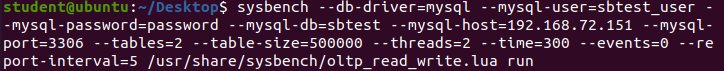
\includegraphics[width=0.80\textwidth]{Appendicies/Test2Command.PNG}
\subsection{VMware results}
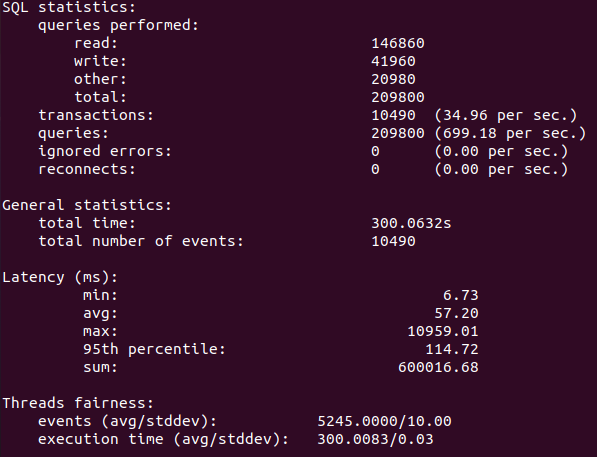
\includegraphics[width=0.80\textwidth]{Appendicies/VMwareTest2.PNG}
\subsection{Docker results}
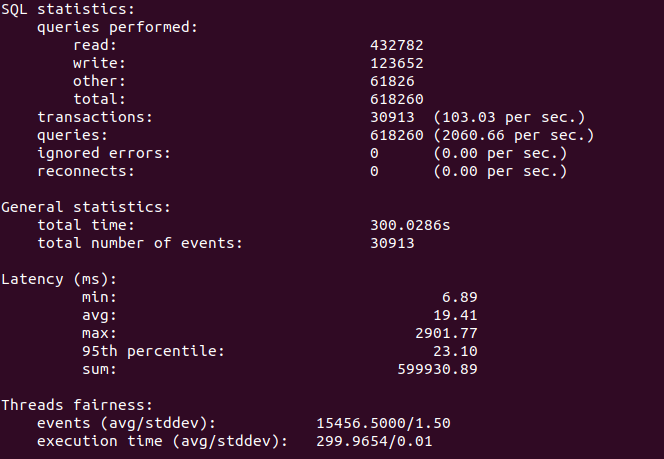
\includegraphics[width=0.80\textwidth]{Appendicies/DockerTest2.PNG}
\section{Test Three - Namebench}
\subsection{VMware Configuration}
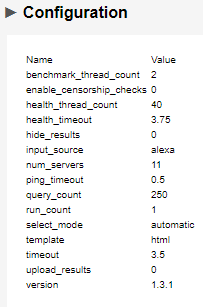
\includegraphics[width=0.40\textwidth]{Appendicies/VMwareTest3Config.PNG}
\subsection{VMware Responses}
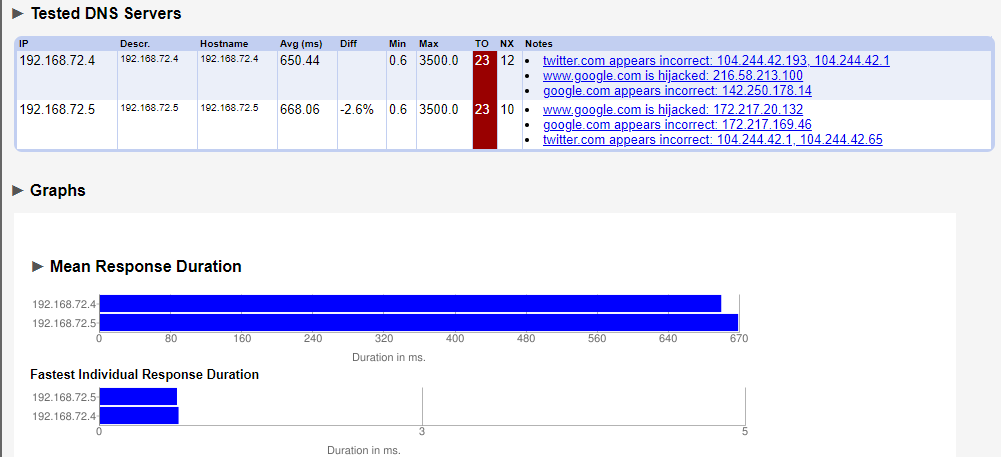
\includegraphics[width=\textwidth]{Appendicies/VMwareTest3Result.PNG}
\subsection{VMware Distribution Chart}
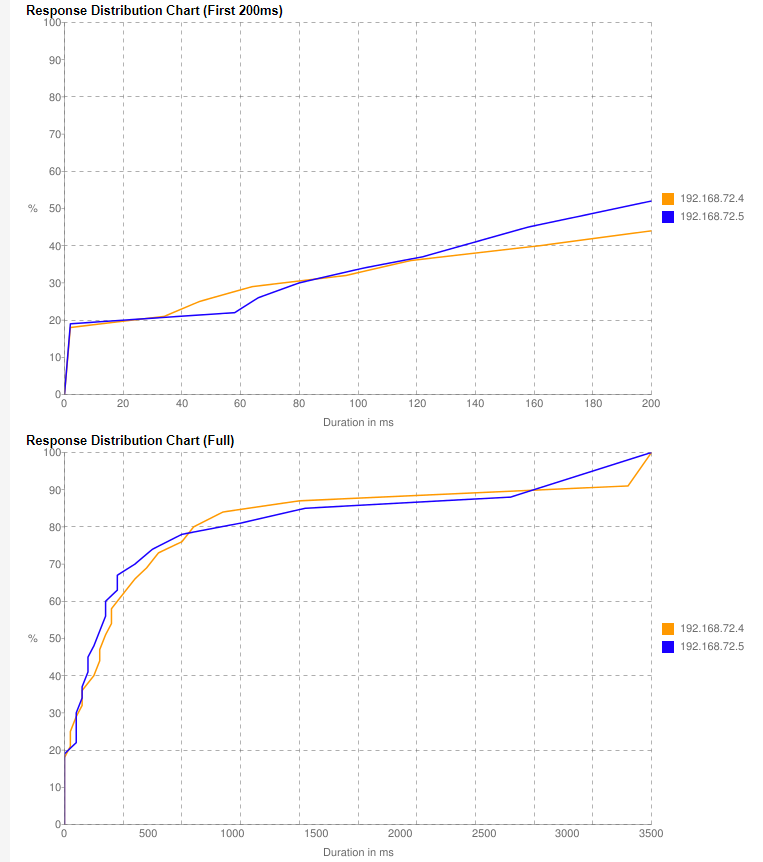
\includegraphics[width=\textwidth]{Appendicies/VMwareTest3Chart.PNG}
\subsection{Docker Configuration}
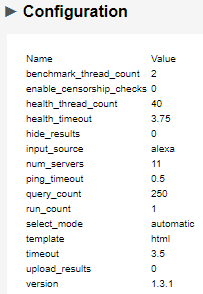
\includegraphics[width=0.40\textwidth]{Appendicies/DockerTest3Config.PNG}
\subsection{Docker Responses}
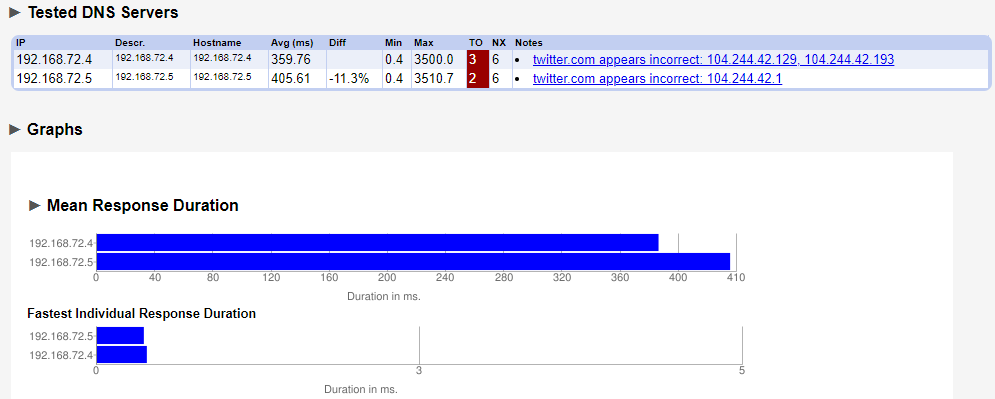
\includegraphics[width=\textwidth]{Appendicies/DockerTest3Result.PNG}
\subsection{Docker Distribution Chart}
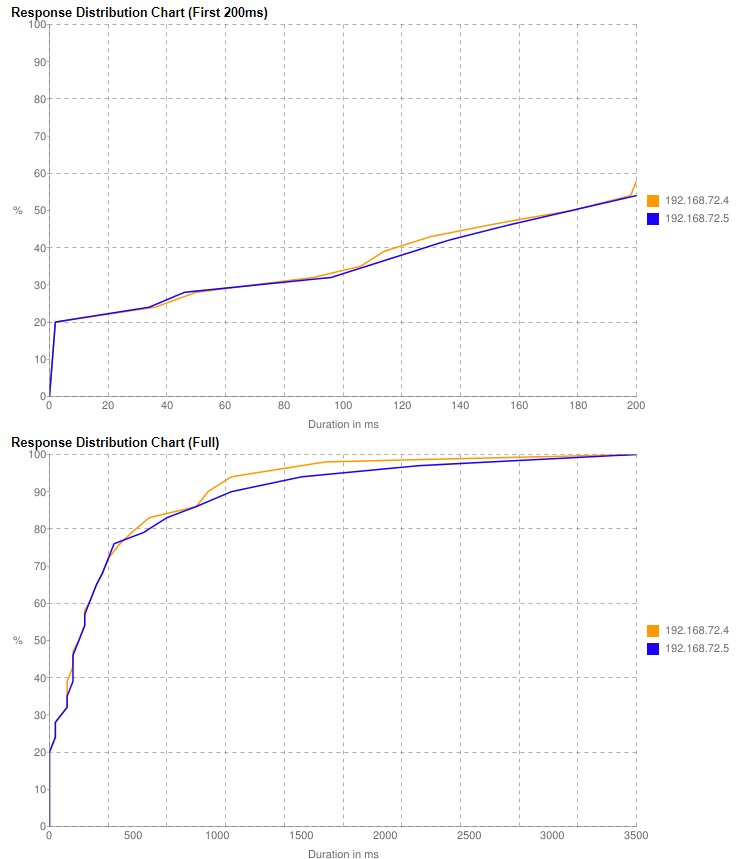
\includegraphics[width=\textwidth]{Appendicies/DockerTest3Chart.PNG}

\section{Test Four}
\subsection{Results}
The testing produced 1000 results for each both VMware and Docker. Important results are already referenced in the synthesis part of this report. Raw data .XLS files were submitted as part of the deliverables for this project.
\end{document}
